\chapter{Implementation of the mem-HNN}

\section{Zielsetzung und Forschungsmethodik}
Upon establishing the precise research methodology, this chapter delves into the practical application of the previously mentioned methods.
First, the analysis phase of the \ac{DSR} process is executed with the goal to establish a model of the research plan 
which the requirements and framework conditions of the \ac{IT}-solution can be derived from. 
Next, the practical implementation is performed during the iterative design phase and uses the method of prototyping.
In the end of the design phase is a functional \ac{IT}-artifact, which fulfills the set requirements.
The evaluation phase in this chapter uses the method of simulation to answer the second part of the research question; to see how efficient 
the \ac{mem-HNN} can utilize the AI-model in terms of throughput and energy usage.

\section{Analysis phase}
\subsection{General conditions}
The first phase of the \ac{DSR}-cycle has the goal of specifying the objective and establishing an according research outline and the requirements of the artifact.
Additionally, the research outline should be visualized as a model of the overall solution concept.\footcite[cf.][278-279]{oesterleKonsortialforschung2010}
The objective of the practical part is already specified in chapter 3.1.
The underlying motivation hereby is to research if the known proof of concepts are feasible on the complete \ac{mem-HNN}
and evaluate if that brings an actual acceleration, which is equivalent to answering the research question of this thesis. 
This is tested by implementing the concept in software that is also part of the ASIC design process.\footnote{cf.\cite{raoUltimateGuideASIC}, p. 1; cf.\cite{ASICDesignFlow}, p. 1}

The implementaton is executed in the programming language Python since it offers a variety of third party libraries that are useful 
for machine learning that are state of the art, like pytorch, scikit learn etc..\footcite[cf.][306-307]{DiscreteContinuousModels}
Furthermore, scikit learn is chosen as machine learning library since it is one of the industry standards for classical machine learning, has a broad variety of features in terms of \ac{RBM}s
and has a lower learning curve compared with e.g. Tensorflow.\footcite[cf.][5-6]{raschkaMachineLearningPython2020}

It should also be clarified that the hardware, which the analog \ac{mem-HNN}-accelerator consists of, is implemented in software. 
This design decision is made out of time constraints of this thesis and part of the ASIC design process before buildng an actual accelerator. 
Nonetheless, the complete hardware is realizable in software without taking compromisses within their functionality.
The simulation data gathered later on is close to the real energy efficiency and throughput.\footcite[cf.][3-4]{hizzaniMemristorbasedHardwareAlgorithms2023} 


Lastly, the energy model used in the simulation can, depending on a specific input, calculate the amount of energy required from the hardware to perform computations.
This energy model is developed by HPE and the Forschungszentrum Jülich.
The explanation for this model is out of scope for this thesis but core parameters are explained to understand the data generation for the energy values.
A seperate paper will be published about the energy model in the near future but kindly for this thesis the model can be used in advance.

\subsection{Requirements}

In order to set requirements for the IT-artifact an ideal overall solution architecture is of importance. 
Hence, a complete solution is modelled, which surpasses both proof of concepts introduced in 2.4.4.
It shows the components required for an acceleration of a \ac{BM} in hardware with the statistical sampling performed by an Hopfield Network, which was never done and tested before.
Furthermore, the following figure\ref{Overall architecture} contains the interaction between the digital computer and the analog mem-HNN Accelerator with five different steps. 
\begin{figure}[H]
    \centering
    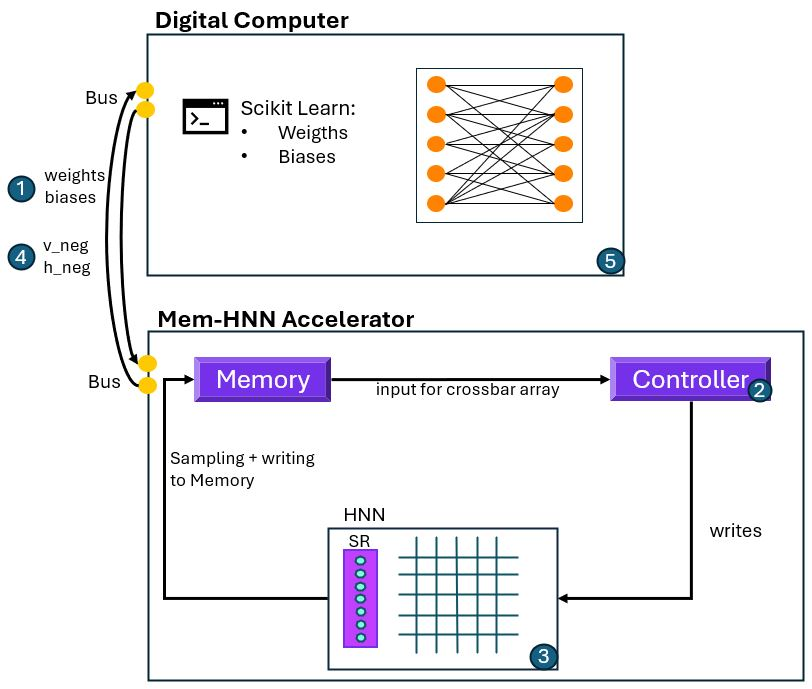
\includegraphics[width=0.80\linewidth]{graphics/Analysemodell.JPG}
    \caption{proposed solution architecture}
    \label{Overall architecture}
\end{figure}
\textbf{1.} contains the initialization of the neural network. 
Hence, the weights and biases are assigned and the structure is build.

\textbf{2.} starts with the transfer of the weigths and biases to the \ac{mem-HNN} accelerator via a bus-system. 
The local memory saves the data and forwards them to the controller. 
The controller is able to programm the memristors in the crossbar array, communicates with the computer and sets a counter and reset for the amount of sampling steps. 

\textbf{3.} is the Hopfield Neural Network (HNN), which contains the memristor crossbar array and the state register (SR).
The state register includes the current neuron configuration.\footcite[cf.][18]{caiHarnessingIntrinsicNoise2019}
For each of the neurons a \ac{TIA} and comparator are required in the hardware.
Furthermore, the state register can lock und unlock specific neurons, so that it is possible to update neurons synchronously.
This enables the possibility of the promissing N/2 update strategy.

\textbf{4.} After iterating over steps two and three multiple times until enough sampling are executed the, all the configurations
of the visible neurons \(v_{neg}\) and the  hidden neurons \(h_{neg}\) are transferred from the controller via the bus-system to
the digital computer. 

\textbf{5.} contains the update of the weights and biases. 
Furthermore, the model can be evaluated in its performance in terms of chosen metrics like prediction accuracy or the negative likelihood etc..
In this case a logistic regression is used for the classification task and the \ac{RBM} is used for the trainng of the neural network. 
After the evaluation the iteration is completed and the new weghts and biases can be transmitted for the following training iteration.

Since such chips do not yet exist, the objective is to construct a simulator pipeline that integrates these individual steps into a simulator, effectively replicating this hardware platform.
Only the bus system, the memory and the controller are not mappable since the local machine already has the hardware.
With this underlying model deriving the requirements is the next step in establishing the research outline.
The aim of generating requirements is to generate good quality, not perfect, requirements that offers an acceptable level of risk to start the project.\footcite[cf.][11]{ebertSystematischesRequirementsEngineering2008}
Hence, these requirements need to cover the functions of the \ac{mem-HNN}, which then must be implemented by the respective software components.
Despite this, requirements may evolve over time and occasionally require adjustments when outcomes differ from initial expectations.
As a result, the analysis of the model in conjunction with the reasearch question and under thought of the defined objective, the following requirements for the software emerged:

\textbf{Digital Computer}
\begin{itemize}
    \item Defining a \ac{RBM}
    \item Utilization of any training data
    \item Training a \ac{RBM}
    \item Establishing a pipeline for the classification
    \item Possibility of conventional sampling algorithms: gibbs sampling and metropolis hasting
    \item Setting individual parameters: sampling steps, training iterations 
\end{itemize}
\textbf{Simulated Mem-HNN Accelerator}
\begin{itemize}
    \item Using any \ac{RBM} as input
    \item Correctly using the Hopfield Network update algorithm
    \item Return sampled output of the neuron configurations 
    \item Correctly using the Hopfield Neural Network as sampling method 
    \item Possibility to use N/2 half updating method instead of asynchronously update of states
    \item Component for measuring the parameters required for evaluation: Speed (throughput) and energy consumption
\end{itemize}
Fruthermore, the python program should be split logically into the different modules and components to enable well structured code. 
With set requirements it is now possible to begin the iterative design and evaluation cycle with focusing on some requirements per iteration.

\section{First Design and Evaluation phase}

This \textbf{Design phase} has the goal of implementing all requirements of the digital computer resulting in a first prototyp iteration.
The first step in the described prototyping methodology within 3.3 is to perform the systemic analysis to categorize the prototype.
In the realm of prototyping, the following categorizations are made: the prototype type (1) is computational, and its fidelity level (2) is high, as it aims to model all functionalities closely to reality.
Furthermore, the complexity (3) is considered moderate because not all hardware components can be modeled in software.
Additionally, the scale (4) remains constant, and there are multiple iterations (5) executed sequentially to train and infer the \ac{RBM}.
The first step, is to chose one of the machine learning libraries like Ternsorflow, Pytorch or Scikit Learn. In this case Scikit Learn is chosen since it is one of the industry standards for classical machine learning, has a broad variety of features in terms of \ac{RBM}s
and has a lower learning curve compared with e.g. Tensorflow.\footcite[cf.][5-6]{raschkaMachineLearningPython2020}
This allows fast development with already well balanced hyperparameters within the library that can be used. 
Another reason is that the available workloads of datasets are popular and devliver results that are comparable with literature.
This is useful to answer the research question in a timely manner with already available functionalities for \ac{RBM}s.
Especially, the implementation of the \ac{RBM} is inspired by an example of the official scikit learn documentation.\footcite[cf.][1]{RestrictedBoltzmannMachine}
In general, the RBM model is modelled as the feature extractor in combination with a logistic regression classifier for the prediction.

Scikit learn offers a variety of datasets that are already in a polished format, ready to use. 
The decision is to use a classification workload of handrwritten digits.
One reason for this is that the load digits dataset is similar to the well known MNIST dataset but has a smaller resolution of 8x8 pixels and features around 1800 samples that can be categorized in 10 classes (integers 0-9).\footcite[cf.][1]{SklearnDatasetsLoad_digits}
The second reason is that the workload is already optimized and therefore can deliver relevant data for the research question.
Also, the dataset can be changed as desired with for example a breast cancer classification workload; in general all datasets that have two states like the activation of neurons in the neural network are compatible.
In this case additionally a nudging of the data is chosen to create more samples, by a factor of five, and to bring more complexity in the workload. 
The split in the dataset is selected to be divided into the conventional 80\% training data and 20\% test data.\footnote{cf.\cite{charithaTypeIIDiabetesPrediction2022a}, p. 1-2; cf.\cite{supriAsianStockIndex2023}, p. 1}

The following task is to set parameters like the learning rate, iterations, size of the hidden layer. 
With having a look in the literature and through testing a learning rate of \(0.2\), 10 training epochs with 72 iterations in one epoch, and an hidden layer of 100 neurons is chosen.
Noteworthy, the size of the visible layer is automatically recognized by scikit learn but since the resolution of the pictures is 8x8 it requires 64 visible neurons to process an input.

The training of the \ac{RBM} is performed in the \texttt{.fit} method and for the functionality to select the preferred sampling algorithm an additional sampling method need to be added.
This process includes modifying the \texttt{\_rbm.py} file in the basic scikit learn library.
The predefined sampling method is gibbs sampling and there is no option to access metropolis hasting within the basic library. 
Therefore, the metropolis hasting alhorithm, explained in 2.2.3 needs to be manually implemented.
The according adjustments are included from the code availability of a paper, which are published in Nature Communiations.\footcite[cf.][11-12]{bohmNoiseinjectedAnalogIsing2022}
This decision was made because the algorithm used there is the original metropolis algorithm by Metropolis et.al..\footcite[cf.][1087-1092]{metropolisEquationStateCalculations1953}
Furtherore, the implementation is performant with many numpy functions. 
To utilize this sampling method, some minor adjustments are made for the user friendliness. 
First, one function is fixed that has a small error, which produced many zero arrays at the beginning of the sampling. 
The user friendliness is achieved by introducing a new parameter \texttt{sampling\_method} that dynamically allows to change the sampling method. 
Another change is the approach of evaluating the performance of the neural network after an x amount of iterations to meassure its performance on the test data while training.
A complete code overview of the metropolis hastings sampling algorithm can be found in the \texttt{mcmc2.py} file as part of the digital delivery with all
adjusted methods for the training of the \ac{RBM} in \texttt{\_rbm.py}, while the overall execution takes place in the \texttt{playground.py}.

Hence, the possibility of different sampling methods are possible and the training of the \ac{RBM} is possible.
To evaluate the results and functionalities the \textbf{Evaluation phase} in this iteration validates the functionalities through a training of the \ac{RBM} with each sampling method and extract their prediction accuracy 
and negative likelihood for each iteration. Following figure\ref{CD_baselines} shows the training results using the gibbs sampling approach. 

\begin{figure}[H]
    \centering
    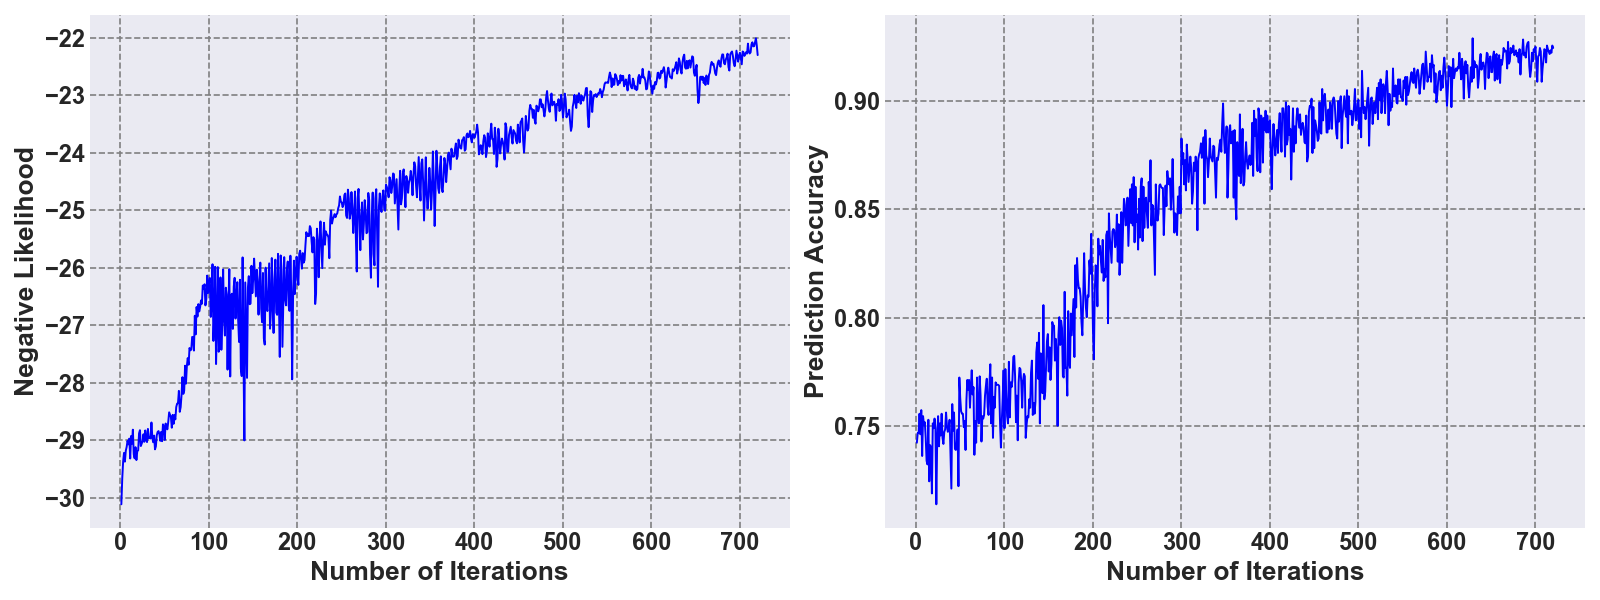
\includegraphics[width=1\linewidth]{graphics/CD_combined_plot.png}
    \caption{Gibbs sampling baselines}
    \label{CD_baselines}
\end{figure}
The right plot shows that the initial prediction accuracy starts at 75\%, akin to that of a linear regression model.
This suggests that without training a linear regression alone could account for this level of accuracy when an untrained \ac{RBM} is included in the pipeline.
Data points are colected after every iteration across the span of 720 iterations. 
It is noteworthy that after 650 iterations the accuracy tagnated and had a maximum prediction accuracy
of 92.29\%. 
In the left plot picturing the negative likelihood, which is a measure of how well a statistical model represents the observed data.
When training a model the aim is to minimize the negative log-likelihood, which means that the model maximizes the probability of generating the observed data.
Hence, it is visible that in the beginning the model learns more rapidly and in steadily grows its knowledge with some smaller break-ins at the end.
The best value is a negative likelihood of -22.01.
\begin{figure}[H]
    \centering
    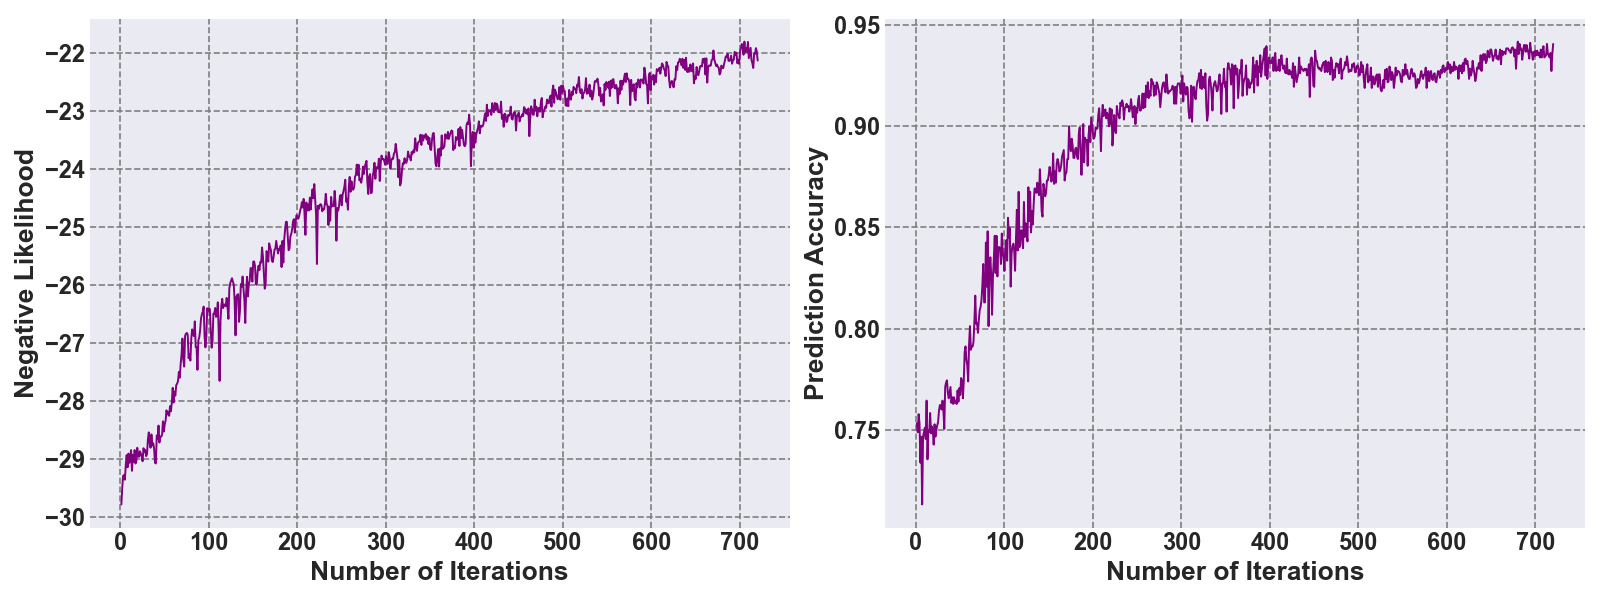
\includegraphics[width=1\linewidth]{graphics/metropolis_combined_plot.png}
    \caption{Metropolis sampling baselines}
    \label{metropolis_baselines}
\end{figure}
In contrast, the figure\ref{metropolis_baselines} used the sampling algorithm of metropolis hasting to train the \ac{RBM}.
Noteworthy is that the prediction accuracy in the right plot has a faster increase in the beginning but already starts to stagnate at around 400 iterations. 
Here, the maximum prediction accuracy already returned 94.15\%. 
The negative likelohood is also growing faster than in gibbs sampling and has less spikes in the beginning showing a more continuously learning rate.
Here, the best negative likelihood value is -21.80.
The gathered data can later on be used as baseline against the desired new updating mehtod of sampling with a Hopfield Network.
Furthermore, the data is comparable and show similar results to those from the literature and are therefore to be considered correct.\footnote{cf.\cite{bohmNoiseinjectedAnalogIsing2022a}, p. 5; cf.\cite{RestrictedBoltzmannMachine}, p. 1}
As a result, with each sampling method successfully undergoing a training, all the functionalities can be proven right and the prototype can be passed 
into the next design iteration.


\section{Second Design and Evaluation phase}

This \textbf{design phase} iteration has the goal of implementating the noisy Hofpield Network as described in the chapter 2.4.4. 
The functionilities of a \ac{RBM} can be reproduced by the Hopfield Neural Network by correctly tuning the noise.
Following subfunctionalities need to be established: imitating the \ac{RBM} activation function, drawing random neurons to update,
correct injection of the gaussian noise scale, calculating the weighted sum,
comparing the weighted sum + bias + noise agaisnt the threshold and saving the new neuron configuration.
Hence, this iteration is accessing new ground since the implementation of the simulator pipline is not validated yet. 

First, a new file \texttt{\_hopfield\_network\_v1.py} is created that aims to first establish a noisy Hopfield Network with a single neuron 
and meassure its activation function.
Like mentioned in 2.4.4, a Hopfield Network has a binary activation function that needs to be made compatible with the sigmoid activation function of the \ac{RBM}.
The Hopfield Network is initialized with a size of just one neuron and an sampling iteration counter of \(1500\) iterations with a thermalization of \(100\) sampling steps before 
the neuron is updated.
The reason for the thermalization is, so that the internal network can get into a flow and do some sampling steps to be statistical independent in order to have un unbiased sampling.
The threshold as defined in the update formula is \(0\). 
As experimented the update formula for implementation of the Hopfield Network looks the following:

\begin{lstlisting}
    for x in range(self.iterations_per_theta):
                    
        self.neuron_index = np.random.randint(0, self.size) #pick a random neuron in the network
        # Calculate the weighted sum for the neuron, excluding its own state
        weighted_sum = sum(self.weights[self.neuron_index][j] * self.configuration[j] for j in range(len(self.configuration)) if j != self.neuron_index)

        self.new_configuration = deepcopy(self.configuration)   #copying the old configuration to create a new one and update it
        if (weighted_sum + self.bias + np.random.normal(0, scale=1.75)) >= self.threshold_theta:          
            self.new_configuration[self.neuron_index] = 1
        else:
            self.new_configuration[self.neuron_index] = 0
            
        self.configuration = deepcopy(self.new_configuration)   #Cloning current configuration and updating the cloned version to the new configuration after comparing with threshold

        if x >= self.thermalization:  
            self.summedConfigurations = self.sum_configurations(self.summedConfigurations, self.new_configuration)    
            self.iterationcounter += 1
        
    self.activationProbabilityPerNeuronDict[self.bias] = self.divide_array_elements(self.summedConfigurations, self.iterationcounter)
    self.bias += 0.025
\end{lstlisting}
In the beginnig a random neuron is drawn to be updated, which currently everytime is neuron number one because the network size is one. 
This allows to meassure the activation probability and fast iteration time with a clear result on how the network behaves. 
Calculating the weighted sum can be seen as the core of the update formula and is done first.
Afterwards to compare against the threshold an bias is added.
The value of the bias ranges from \(-6; 6\) in step sizes of \(0.025\). After completing all samplin iterations beginning with \(-6\) the step size is added to the bias until all iterations are made.
This is sufficient for the neuron activation function of an ordinary Hopfield Network and results in the binary step. 
The resulting activation function is obtained by summing all configurations within a single bias configuration.
In a next step, the configurations counted are divided by the number of total sampling iterations within the bias configuration (in this case 1500 iterations).
That following figure \ref{Noisy_acitivation_function_bad} \textbf{Evaluates} the resulting activation probability of the single neurons. 
\begin{figure}[H]
    \centering
    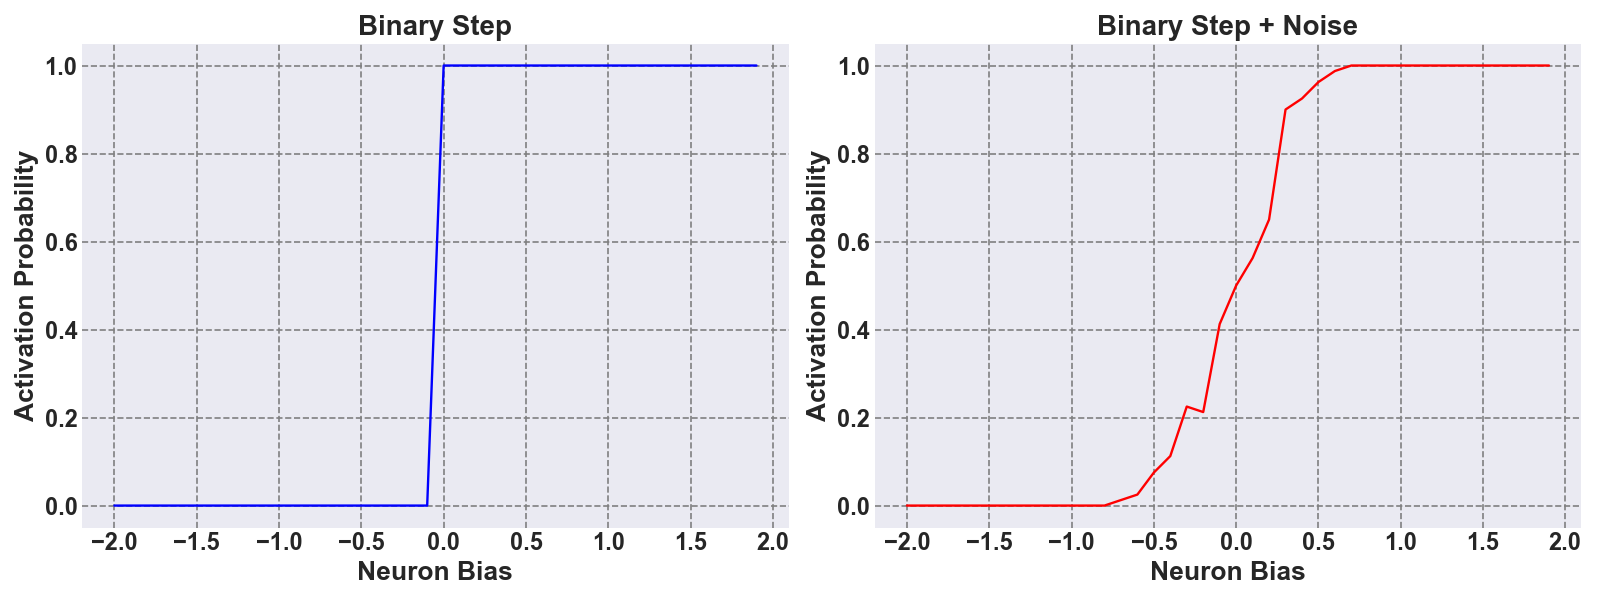
\includegraphics[width=1\linewidth]{graphics/combined_noise_activation_plots.png}
    \caption{Modification of the the Hopfield Network binary step activation function}
    \label{Noisy_acitivation_function_bad}
\end{figure}
In the left plot, visualized in blue, the activation probability of the neuron is shown without adding noise to the plot. 
The behaviour is like sme would expect it; once the bias reaches 0 the neuron is activated all the time.
Far more interesting is the red plot on the right side, which introduces some noise into the binary step function, bringing it closer to the logistic sigmoid activation function used in the \ac{RBM}.
To achieve this behavior, injecting noise through a Gaussian normal distribution can modify the activation function, making it compatible with the sigmoid function.\footnote{cf.\cite{bohmNoiseinjectedAnalogIsing2022}, p. 1-2; cf.\cite{mahmoodiVersatileStochasticDot2019}, p. 2}
Technically this is performed by adding \texttt{np.random.normal(0, scale=1.75)} to the weighted sum and the bias, with 0 beeing the mean of the distribuion and the scale representing the standard deviation. 
Hereby, it is important to find a standard deviation that is very close to the true activation probability is important, otherwise the training of the RBM would not work.
In addition to that, the standard deviation changes with neuron size and needs to be readjusted if changes are made to the networks structure.

The right plot shows that the noise injection works, even though it doesn't perfectly copy the sigmoid function.
Concluding from this the sigmoid function is not achieved and the trainig of an \ac{RBM} probably fails. 
Therefore, to completely evaluate and ensure that the injected noise fits to the logistic sigmoid function, the function itself is plotted 
as index, to have a visual comparison. 
Now, finding the correct standard deviation is the goal. 
In following figure\ref{Noisy_acitivation_function_good} the hyperparameter is tuned and the resulting scale is visualized.
It verifys that a noisy activation function of a Hopfield Network can imitate the sigmoid function of a \ac{RBM} correctly:
\begin{figure}[H]
    \centering
    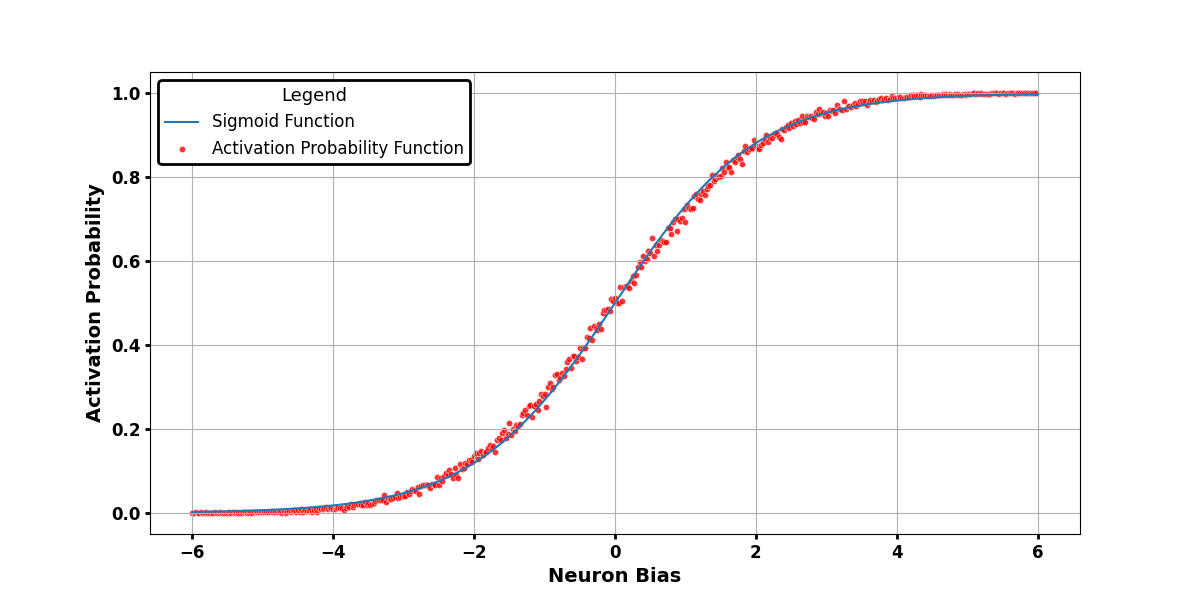
\includegraphics[width=1\linewidth]{graphics/Noisy_HNN_2.png}
    \caption{Noisy activation function of the Hopfield Network imitating the \ac{RBM}}
    \label{Noisy_acitivation_function_good}
\end{figure}
\section{Third Design and Evaluation phase}

Now, that the proof of concept has been validated, this \textbf{Desing Phase} has the goal of connecting the 
Hopfield Network as a sampling method to the \ac{RBM} and therefore enable a complete training. 
This includes using the weights and biases of the \ac{RBM} as an input and performing the sampling with the input.
Finally, the sampled output of the visible and hidden neuron configurations need to be returned, so that the digital computer can update the weights.
With these subgoals the total goal is to enable a complete training of the \ac{RBM} with the sampling method of the Hopfield Network. 
Furthemrore, if the training is successful, the possibility of the N/2 half updating method instead of asynchronously updating of the states should be implemented.
The first technical step is to extend the \texttt{\_rbm.py} to fit the new sampling method: 
\begin{lstlisting}
        if sampling_method == SamplingMethod.GIBBS:
                v_neg = self._sample_visibles(self.h_samples_, rng)
                h_neg = self._mean_hiddens(v_neg)

        elif sampling_method == SamplingMethod.METROPOLIS_HASTING:
            h_neg,v_neg=mcmc_sample(10000,len(self.components_))

        elif sampling_method == SamplingMethod.HOPFIELD_NETWORK:  
            # Hopfield Network Sampling
            v_neg, h_neg = interface_hopfield_sampling(self.components_, self.intercept_visible_, self.intercept_hidden_, iterations_per_theta, N2_HALF=False)    
\end{lstlisting}
Here, the compontents represent the weights of the neurons in the network, while intercept\_visible and intercept\_hidden represent the bias of the neurons. 
Within the, hopfield\_network\_interface\_v2.py, the parameters are taken and an object of the class is initiated. 

\begin{lstlisting}
    def interface_hopfield_sampling(components_, intercept_visible_, intercept_hidden_):
   
        H_net = Hopfield_Net(components_, intercept_visible_, intercept_hidden_)
        H_net.update_network_state()
        
        return H_net.v_neg , H_net.h_neg
\end{lstlisting}
Inside the class, the initialization of all the parameters and weights are performed. 
The update formula needs to calculate the weighted sum, which necessarily requires to know all the weights between the neuron itself, to all the other neurons. 
The decision is to create a weight matrix shown in \ref{attachement:weight_matrix}. 
The function begins by defining the total number of hidden and visible neurons based on the class properties parameters used as input.
These quantities dictate the dimensions of the weight matrix, which, in this instance, results in a matrix of size (100, 64).
This square matrix represents the fully interconnected network, where each neuron can potentially connect to every other neuron, including itself.
As mentioned in 2.2.3, the diagonal elements (self-connections) are set to zero in \ac{RBM}s.

Another important aspect is to maintain the model's symmetry, which is crucial for the energy-based nature of RBMs and the dynamics of Hopfield networks.
Hence, for this reason and simplicity, the weight matrix is initialized as a symmetric matrix using NumPy's np.zeros function.
This ensures that all initial weights are set to zero before being explicitly defined through the components weights.
Scikit Learn randomly initializes the weights by default close to zero, while the biases are set to zero. 
This small weights allow to support an effective gradient distribution which protects against rapid saturation or inefficient learning,
while the bias set to zero allows the network to begin in a neutral position and learn on its own. 

The subsequent nested loops iterates over the indices for hidden and visible neurons to fill the weight matrix.
For each pair of hidden and visible neurons, the corresponding weights are extracted from the components matrix.
This matrix essentially serves as the template for the interactions between hidden and visible layers.
Indexing within the weight matrix is handled carefully, to respect the structure of the RBM. 
Therefore, the decision is to set weights between a hidden neuron i and a visible neuron j at positions \texttt{[i, j+num\_hidden]} and \texttt{[j+num\_hidden, i]} to ensure symmetry.

With some more adjustments necessary to the code the first training of the \ac{RBM} with the sampling method of the Hopfield Network can begin. 
The Hyperparmeters first are set to the same scale(1.75) and same thermalization(100) as for a single neuron but with more sampling steps (5000 sampling steps) than before. 
The results of the traning are visualized in figure\ref{HNN_training}.
\begin{figure}[H]
    \centering
    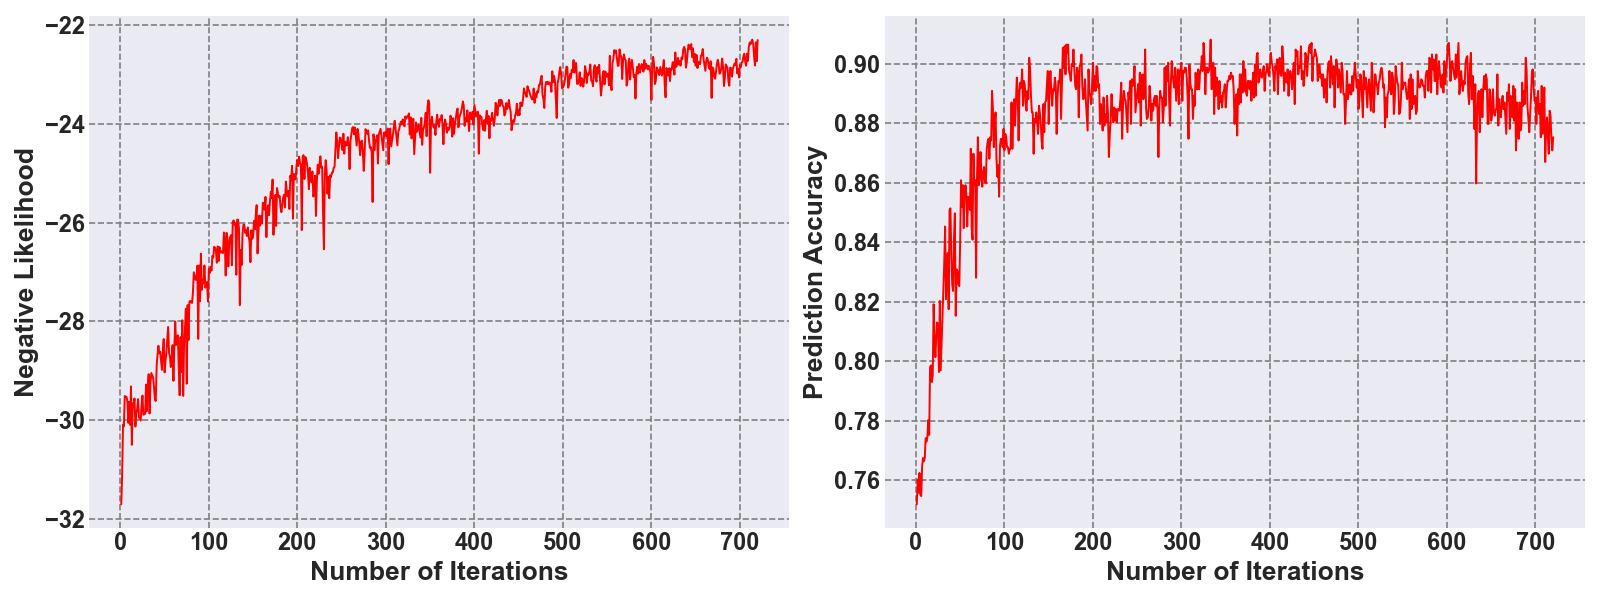
\includegraphics[width=1\linewidth]{graphics/HNN_combined_plot.png}
    \caption{Hopfield Network sampling baselines}
    \label{HNN_training}
\end{figure}
First of all, it can be recognized that the training was successful, which was uncertain. 
Noteworthy, that with this method the output had to be transposed to be able to parse the data Scikit Learn.
In a second look it can be seen that the negative likelihood is far more stable as gibbs sampling and rather has similarities with metropolis hastings sampling.
Here, the best value is a likelihood of -22.3, so slightly worse than metropolis hastings and gibbs sampling. 
The right plot showing the prediction accuracy has the highest ascent of all the three graphs, which proofs that the 
less iterations are required to receive good results compared to the other two methods.
Still, The best prediction value is 90.81\% and therefore worse than gibbs and metropolis hastings. 
The reason for this can be the hyperparameter tuning.
Since the noisy Hopfield Network method can become sensitive fast or is not adjusted correctly 
for this amount of neurons in the network, receiving this result without further adjustments already looks promissing. 

As a result, the following hyperparameters are tuned to possibly received better outcomes. 
Specifically, the scale, which represents the standard deviation and is used as noise is tuned. 
In addition to that the amount of sampling iterations within a single training iteration is tuned.
One extended parameter could be the learning rate and the total iterations but to have an appropriate benchmark against the other two 
sampling methods these parameters are locked in. 
Last but not least, the possibility of tuning the thermalization could help out too even if slightly less significant than the other two hyperparameters.
Since the training takes around 40 minutes to complete tuning too many hypaerparameters takes too much time for the period of this thesis. 
First hyperparameter researched is the influence of the standard deviation (scale) to the maximum prediction accuracy. 
Especially the maximum prediction accuracy of the last 50 training iterations are gathered since this is the relevant area for inference.
Given that the Hopfield Network operates as a statistical sampling method, the standard deviation is also calculated for these final 50 training iterations.
This is done for the scale range of 1.0 to 2.0 within step sizes of 0.05, totalling to 21 single trainings done.
The result is illustrated in figure\ref{Hyperparamers_Scale_ohne}:
\begin{figure}[H]
    \centering
    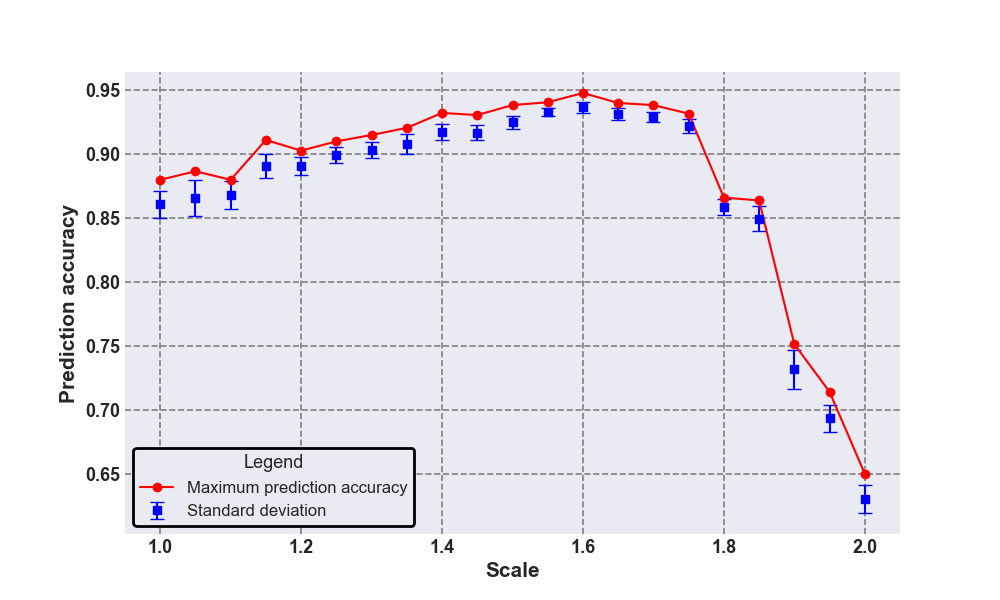
\includegraphics[width=0.9\linewidth]{graphics/NEW_Scale_Ohne_N2_Half_Pred_Acc.png}
    \caption{Hopfield Network Hyperparametertuning scale}
    \label{Hyperparamers_Scale_ohne}
\end{figure}
The result shows that beginning with a scale of 1.0 the prediction accuracy slowly rises until the scale of 1.6
Here, the maximum value is 94.77\% and with that surpasses the performance of both metropolis hastings and gibbs sampling. 
After a scale of 1.75 the prediction accuracy falls off a cliff indicating that the activation function of the \ac{RBM} is not modelled correctly anymore.
This shows that depending an network size and workload the adjustment within this method is important to achieve good results. 
The standard deviation follows the maxmimum prediction accuracy pretty closely and has no outliers indicating that the prediction accuracy is only a lucky random training.
Close to the sclae of 1.0 the deivation is slightly lower compared to the rest of the plot, showing that the scale could be too low to model the sigmoid function correctly. 

In a next step, the best fit with a scale of 1.6 is used for the second hyperparameters. 
The sampling iterations within one training iterations are now tuned.
Hence, the decision is to begin with 1000 sampling iteration continiunig with an increase of 1000 iterations until 15000 iterations are reached. 
With that the training showed that the interesting are is around 1000 to 4000 iteration and that the step size of 1000 is too big for that. 
To be more granular two extra trainings with iterations 1500 ad 2500 werde completed, totalling to 17 trainings performed.
The values are extracted as before, by considering the last 50 iterations and then calculating both the maximum value and the standard deviation from this subset.
The visualized results can be found in following figure\ref{Hyperparamers_Iteraions_ohne}:
\begin{figure}[H]
    \centering
    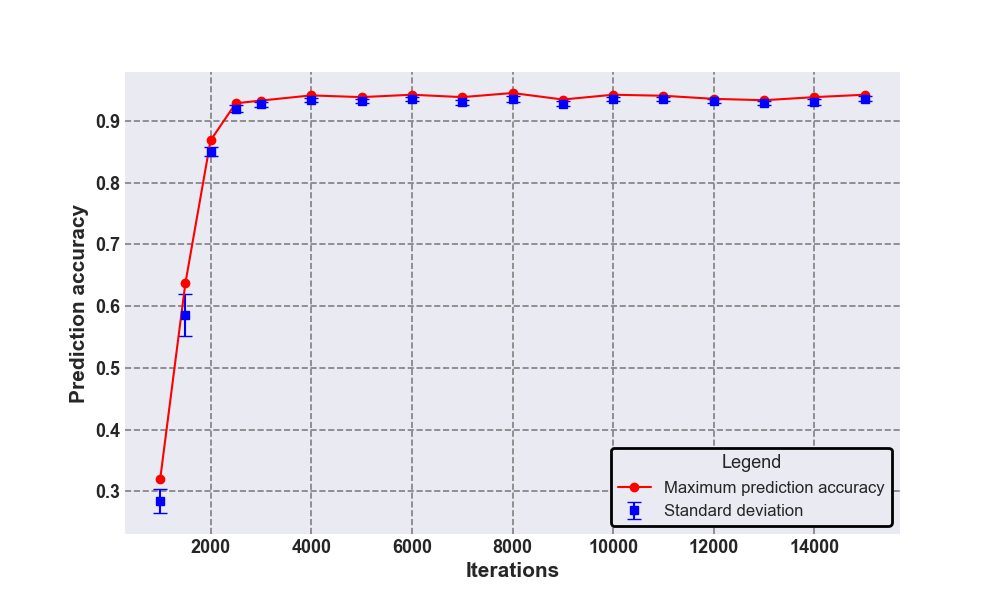
\includegraphics[width=0.9\linewidth]{graphics/Iterations_Ohne_N2_Half_Pred_Acc.png}
    \caption{Hopfield Network Hyperparametertuning sampling iterations}
    \label{Hyperparamers_Iteraions_ohne}
\end{figure}
The line of maximum prediction accuracy starts at the first iteration with a value close to 0.3 and rises rapidly to reach a value just above 0.92 after around 2500 iterations.
From the point of 4000 iterations onwards, the accuracy remains largely constant with slight fluctuations.
The best value is at 15000 iterations with an prediction accuracy of 94.5\%, while at 4000 iterations the accuracy is at 93.35\%.
The error bars indicating the standard deviation are large at the beginning of the graph, which indicates that not enough neurons were updated in the sampling process.
However, with the number of iterations increasing, the error bars become smaller resulting in a more stable accuracy.
Key take away is that after 4000 iterations there are no significant changes to the outcome of the prediction accuracy.

With the successful training and tuned hypaerparameters in the next step the possbility of the N/2 half updating methdod should be researched already mentioned in 2.4.3 and 3.1.
N/2 half is updating neurons synchronously instead of the conventional asynchronously (only one neuron is chosen and updated) used in the Hopfield Network updating mechanism.\footcite[cf.][23-24]{caiHarnessingIntrinsicNoise2019}
Following adsjustments are made in the code to achieve this behaviour:
\begin{lstlisting}
    self.neuron_index = np.random.randint(0, 2, self.size) #pick complete random neurons in the network, result [0,1,1,0] and so on for size of the network

                weighted_sum = np.dot(self.weights[:, :], self.configuration)   
                self.new_configuration = deepcopy(self.configuration)
                bias = self.bias 

                for i in range(len(self.neuron_index)):              
                    #updating function comparing against threshold
                    if self.neuron_index[i] > 0:
                        if (weighted_sum[i] + bias[i] + np.random.normal(0, scale=self.scale)) >= self.threshold_theta:          
                            self.new_configuration[i] = 1
                        else:
                            self.new_configuration[i] = 0
\end{lstlisting}
The neuron index now assigns either a 1 or a 0 to each neuron, with 1 meaning that the sum of this neuron is calculated and will be compared against the threshold. 
In a completely random process this would about lead to 25\% of all neurons updated (\(50\% drawn * 50\% updated\)).
To create a good comparison, the same parameters scale and sampling iterations are tuned for this updating method. 
In this method, 21 complete training sessions are also carried out for this purpose.
Beginning with the scale the result is visualized in figure\ref{Hyperparamers_Scale_mit} :
\begin{figure}[H]
    \centering
    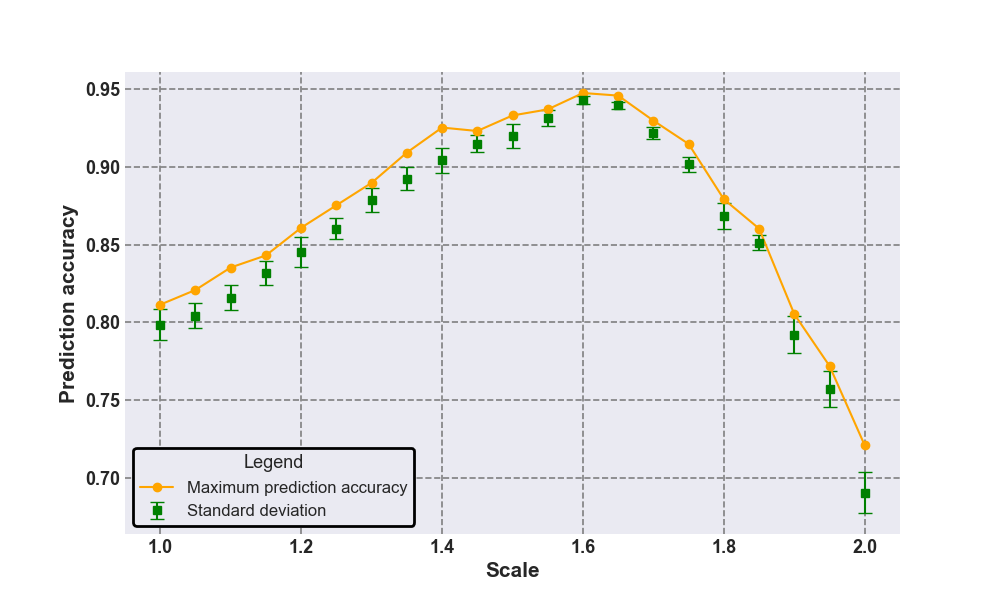
\includegraphics[width=0.9\linewidth]{graphics/NEW_Scale_MIT_N2_Half_Pred_Acc.png}
    \caption{Hopfield Network Hyperparametertuning scale for N/2}
    \label{Hyperparamers_Scale_mit}
\end{figure}
On a first glance, the prediction accuracy beginning from left to right is constantly rising until it reaches the scale of 1.6.
Here, the maximum prediction accuracy tops out at 94.76\%.
What is interesting, that in \ref{Hyperparamers_Scale_ohne} the exact same scale has also the best performance. 
With increasing the scale after the top of 1.6, the accuracy falls off a cliff. 
Noteworthy, is that in comparison with \ref{Hyperparamers_Scale_ohne} the N/2 half updating method has nearly equal prediction accuracy
but is more sensitive. 
This means that the configuration of the hyperparameters is tougher for this updating method and results can get worse more easily. 
The standard deviation represented in the error bars is high at the lower scale values validating that the sigmoid function is not properly mapped. 
This is similar for too high values beginning at a scale of 1.8.

The second hyperparameter are the amount of sampling iterations required to achieve good results. 
In the training process the plan is to begin with the same step sizes like earlier on. Soon it was clear,
that the granularity needs to be much finer too achieve good results. 
Therefore, the decision is to start at iteration 201 (1st iteration after the 200 thermaliation steps) and ending with a sampling iteration of 250 with a step size of 1.
This totals to 50 complete training sessions. The new results are illustrated in figure\ref{Hyperparamers_Iteraions_mit}:
\begin{figure}[H]
    \centering
    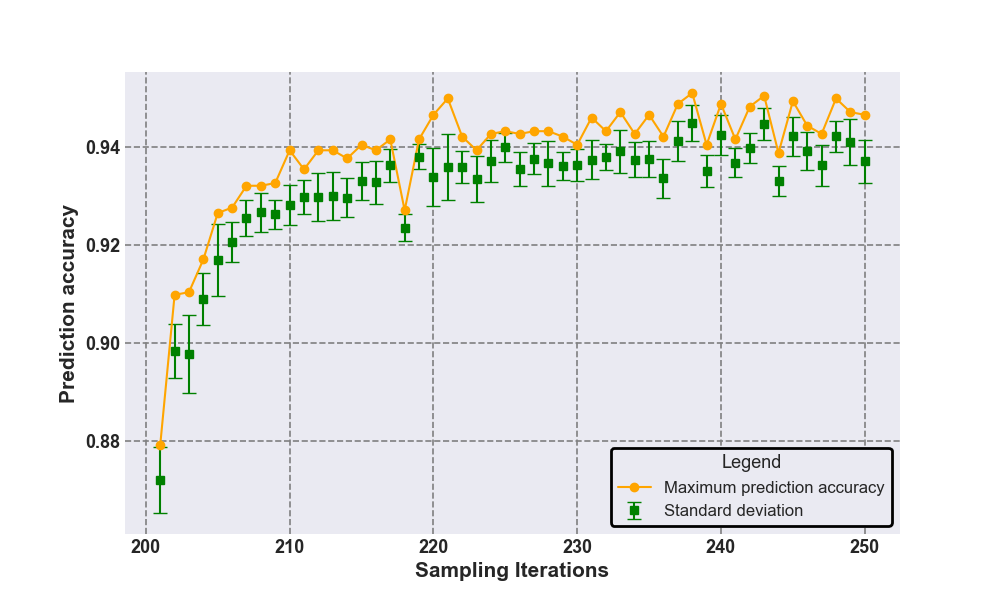
\includegraphics[width=0.9\linewidth]{graphics/Iterations_MIT_N2_Half_Pred_Acc.png}
    \caption{Hopfield Network Hyperparametertuning sampling iterations for N/2 half}
    \label{Hyperparamers_Iteraions_mit}
\end{figure}
The figure shows that with only 10 sampling iterations after the thermalization good prediction accuracies of 94\% can be achieved. 
The maximum prediction value is 95.10\% at 221 sampling iterations, which surpasses the earlier achieved results.
Nonetheless, the key message here is that far less sampling iterations are needed within one big training iteration of the \ac{RBM}
to achieve good results. 
When comparing the number of 221 to the around 4000 sampling iterations required in \ref{Hyperparamers_Iteraions_ohne} it would be more efficient by a factor of 
\(18.09x\). In return, this updating methods saves time and also has less energy consumption required.

With this third design and evaluation phase ending all the functionalities of the prototype are implemented and the prototype itself is complete. 

\section{Final Evaluation phase}
In this final evaluation phase the functional prototype should now be validated within the evaluation phase of the \ac{DSR} framework.
The goal is to answer the research question ``Can Boltzmann Machines be \textbf{efficiently} implemented on physics-inspired
Hardware accelerators by analog noise injection?''.
Since the key word here is efficiently, a simulation will be performed to meassure the parameters required for evaluation.
With the model purpose set, the model scope(time frame) of the simulation introduced in 3.4 is to be considered as short with only mutliple weeks and only one person working on the simulation. 

The next step is to define the result variables. The two variables that are of interest in literature to meassure the performance of the
\ac{mem-HNN} accelerator are troughput (samples/sec) and energy consumption (energy/operation). 
These two metrics are widely used in literature and can create a good comparison.\footnote{cf.\cite{bellettiJanusFPGABasedSystem2009}, p. 54-55; cf.\cite{aaditAcceleratingAdaptiveParallel2023}, p. 1-2; cf.\cite{ortega-zamoranoFPGAHardwareAcceleration2016}, p. 16-17}
Hereby, throughput can be defined as the time needed per Hopfield cycle (sampling iteration) per second.\footcite[cf.][6-7]{bohmNoiseinjectedAnalogIsing2022} 
Meanwhile, the energy consumption is defined by summing over all the single energy consumptions within one sampling iteation.
The resulting unit is called energy/operation. 

Now that the result variables are set the input parameters neeed to be clarified. 
For the throughput knowledge about the autocorrelation of the sampling is required.
Autocorrelation is a statistical measure that captures the degree of correlation between successive configurations generated by timeseries, in this case sampling algorithm for the training of a \ac{RBM}.\footcite[cf.][1-6]{tanakaReductionAutocorrelationHMC2017}
Long correlations between configurations can reduce the effective sample size and lead to inefficiency impacting the precision of the model.
This is important for the result variable ``troughput'' because it allows to know when the sampling is statistically independent and ready to use and therefore how many sampling iterations neeed to be done for an effective training. 
The equation to calculate the statistical dependency of 2 successive samples is the auto-covariance function: 
\begin{equation}
    K_{XX}(t_1, t_2) = \mathbb{E}[(X_{t_1} - \mu_{t_1})(X_{t_2} - \mu_{t_2})] = \mathbb{E}[X_{t_1} X_{t_2}] - \mu_{t_1}\mu_{t_2},
\end{equation}
with \(t_1,t_2\) being two distinct points in time and \(X_{t1},X_{t2}\) are random variables representing the values of the stochastic process at the distinct time points. 
\(\mu_1,\mu_2\) are the mean (expected) values of the random variables \(X_{t1},X_{t2}\). 
The \(\mathbb{E}\) is an expectation operator and is used to calculate the expected value of the expression within the brackets.
Also, the cycle speed of the \ac{mem-HNN} accelerator is needed. 
The clock frequency is around 700MHz and therefore can sample 700 million samples per second, which is about 1.44ns for a single clock cylce.\footcite[cf. table1][7-8]{caiPowerefficientCombinatorialOptimization2020} 
Noteworthy, these numbers are takem from a neural network with 111 neurons. 
On the other hand, the only input variable for the energy consumption is the energy model of the \ac{mem-HNN}, which is introduced in 4.2.1 and is developed by HPE in combination with the Forschungszentrum Jülich.
This allows to meassure each of the individual energy consumptions that are configured to the specifications of the \ac{mem-HNN} hardware accelerator.\footcite[cf.][1-5]{hizzaniMemristorbasedHardwareAlgorithms2023}
For both of the methods one input of course is the finished prototype, that mirrors the functionalities of the \ac{ASIC} on a high level.

With the simulation model specified, the autocorrelation can be implemented into the prototype. 
The decision is to average the values of the output configurations from row to row to an average of 60.
This allows to extract a smoother autocorrelation plot that is not too biased in terms of the statistical approach.
In the attachment\ref{attachement:autocorrelation} the full implementation of the autocorrelation function is available.
To compare the performance of the individual sampling methods in terms of the autocorrelation a threshold is required. 
Here, \(1/\mathrm{e}\) is chosen since it is inspired by many fields, like physics(diffusion length), chemistry and mathematics(half-life as a threshold) etc..\footnote{cf.\cite{archieStatisticalAnalysisHeterozygosity1985}, p. 624-630; cf.\cite{bohmNoiseinjectedAnalogIsing2022}, p. 7-13}
Folliwng results are visualized in following figure\ref{Autocorr comparison}:
\begin{figure}[H]
    \centering
    \includegraphics[width=1\linewidth]{graphics/Visualisierungen_Autocorr_individual_7.png}
    \caption{Autocorrelation for the three sampling methods}
    \label{Autocorr comparison}
\end{figure}

The first row shows the conventional \textbf{Metropolis Hastings} sampling method. On the right plot the autocorrelation
and the according sampling steps are visualized. It can be seen, that the value falls below the threshold at around \textbf{100 sampling steps}, 
Falling below the threshold of \(1/\mathrm{e}\) symbolizes that statistical independent samples are generated.
The left plot therefore meassures the first sampling step within each training iteration that falls below this threshold. 
Here, named correlation time. It can be seen that the the scale on the x-axis in the left plot is higher compared to the other two sampling approaches, 
meaning that metropolis hastings is \textbf{more sensitive}. 

The second row is the \textbf{single neuron Hopfield Network} sampling approach. 
In the right plot it shows that the autocorrelation threshold is reached around after around \textbf{200 sampling steps}.
Even if the value is \textbf{2x worse} than with metropolis Hastings the correlation time for the whole training is \textbf{more stable}.
So even if the initial autocorrelation takes longer over a whole training period the end result has an \textbf{better average} than Metropolis Hastings.

The last approach is the \textbf{N/2 half Hopfield Network}. 
The result verifys the new methods right to exist with only about \textbf{3 iterations} to surpass the threshold in the right plot.
Furthermore, the methods correlation time in the left plot shows that it is by far more \textbf{stable} than the other 2 approaches.
When setting this into perspective even with a conservative average of 5 iterations as correlation time, N2/Half updating therefore
performs \textbf{40x better}, than the single neuron Hopfield Network and \textbf{20x better} than Metropolis Hastings.
When comparing the correlation at the end of the traing iterations, the performance even increases: \textbf{34x better} than the single neuron Hopfield Network (correlation time value of 170) and \textbf{46,6x better} than Metropolis Hastings (correlatin time value of 233).
Surprisingly for this updating method large statistical dependency could be seen in two out of the 720 training iterations.
This means that for these two iterations the autocorrelation \textbf{doesn not fall under the threshold} of \(1/\mathrm{e}\).
The training was attempted three times, and in each instance, the phenomenon occurred between iterations 300 and 500.
Still, this has no impact on the performance of the training and therefore can be seen as outlier.
It is open for further research to identify why this doesn not happen with the other two approeaches and what is the cause.
Since the correct value for not falling under the threshold would be infinity the scale in the plot would be too large. 
Therefore, the same plot with these two outliers can be found in the attachment\ref{attachement:autocorrelation_errors}.

After identifying the autocorrelation of the desired metric, "throughput," it can be calculated by combining the autocorrelation with the cycle speed of the \ac{mem-HNN}.
This is done by taking the autocorrelation time of both Hopfield Network approaches (with N/2 Half and without) and mutlitplying them with the cycle time of the \ac{mem-HNN}.
In addition to that the inverse of the result is calculated resulting in the desired throughput metrics `` samples/second''.
Noteworthy, the cycle time for the \ac{mem-HNN} is 1.44ns for 111 neurons in the network. 
Because the network in this thesis has 164 neurons, the time used for the calculation is estimated to be about 2ns, which can be seen as conservative estimate.
The subsequent visualization\ref{Throughput comparison} shows the throughput for the Hopfield Network:
\begin{figure}[H]
    \centering
    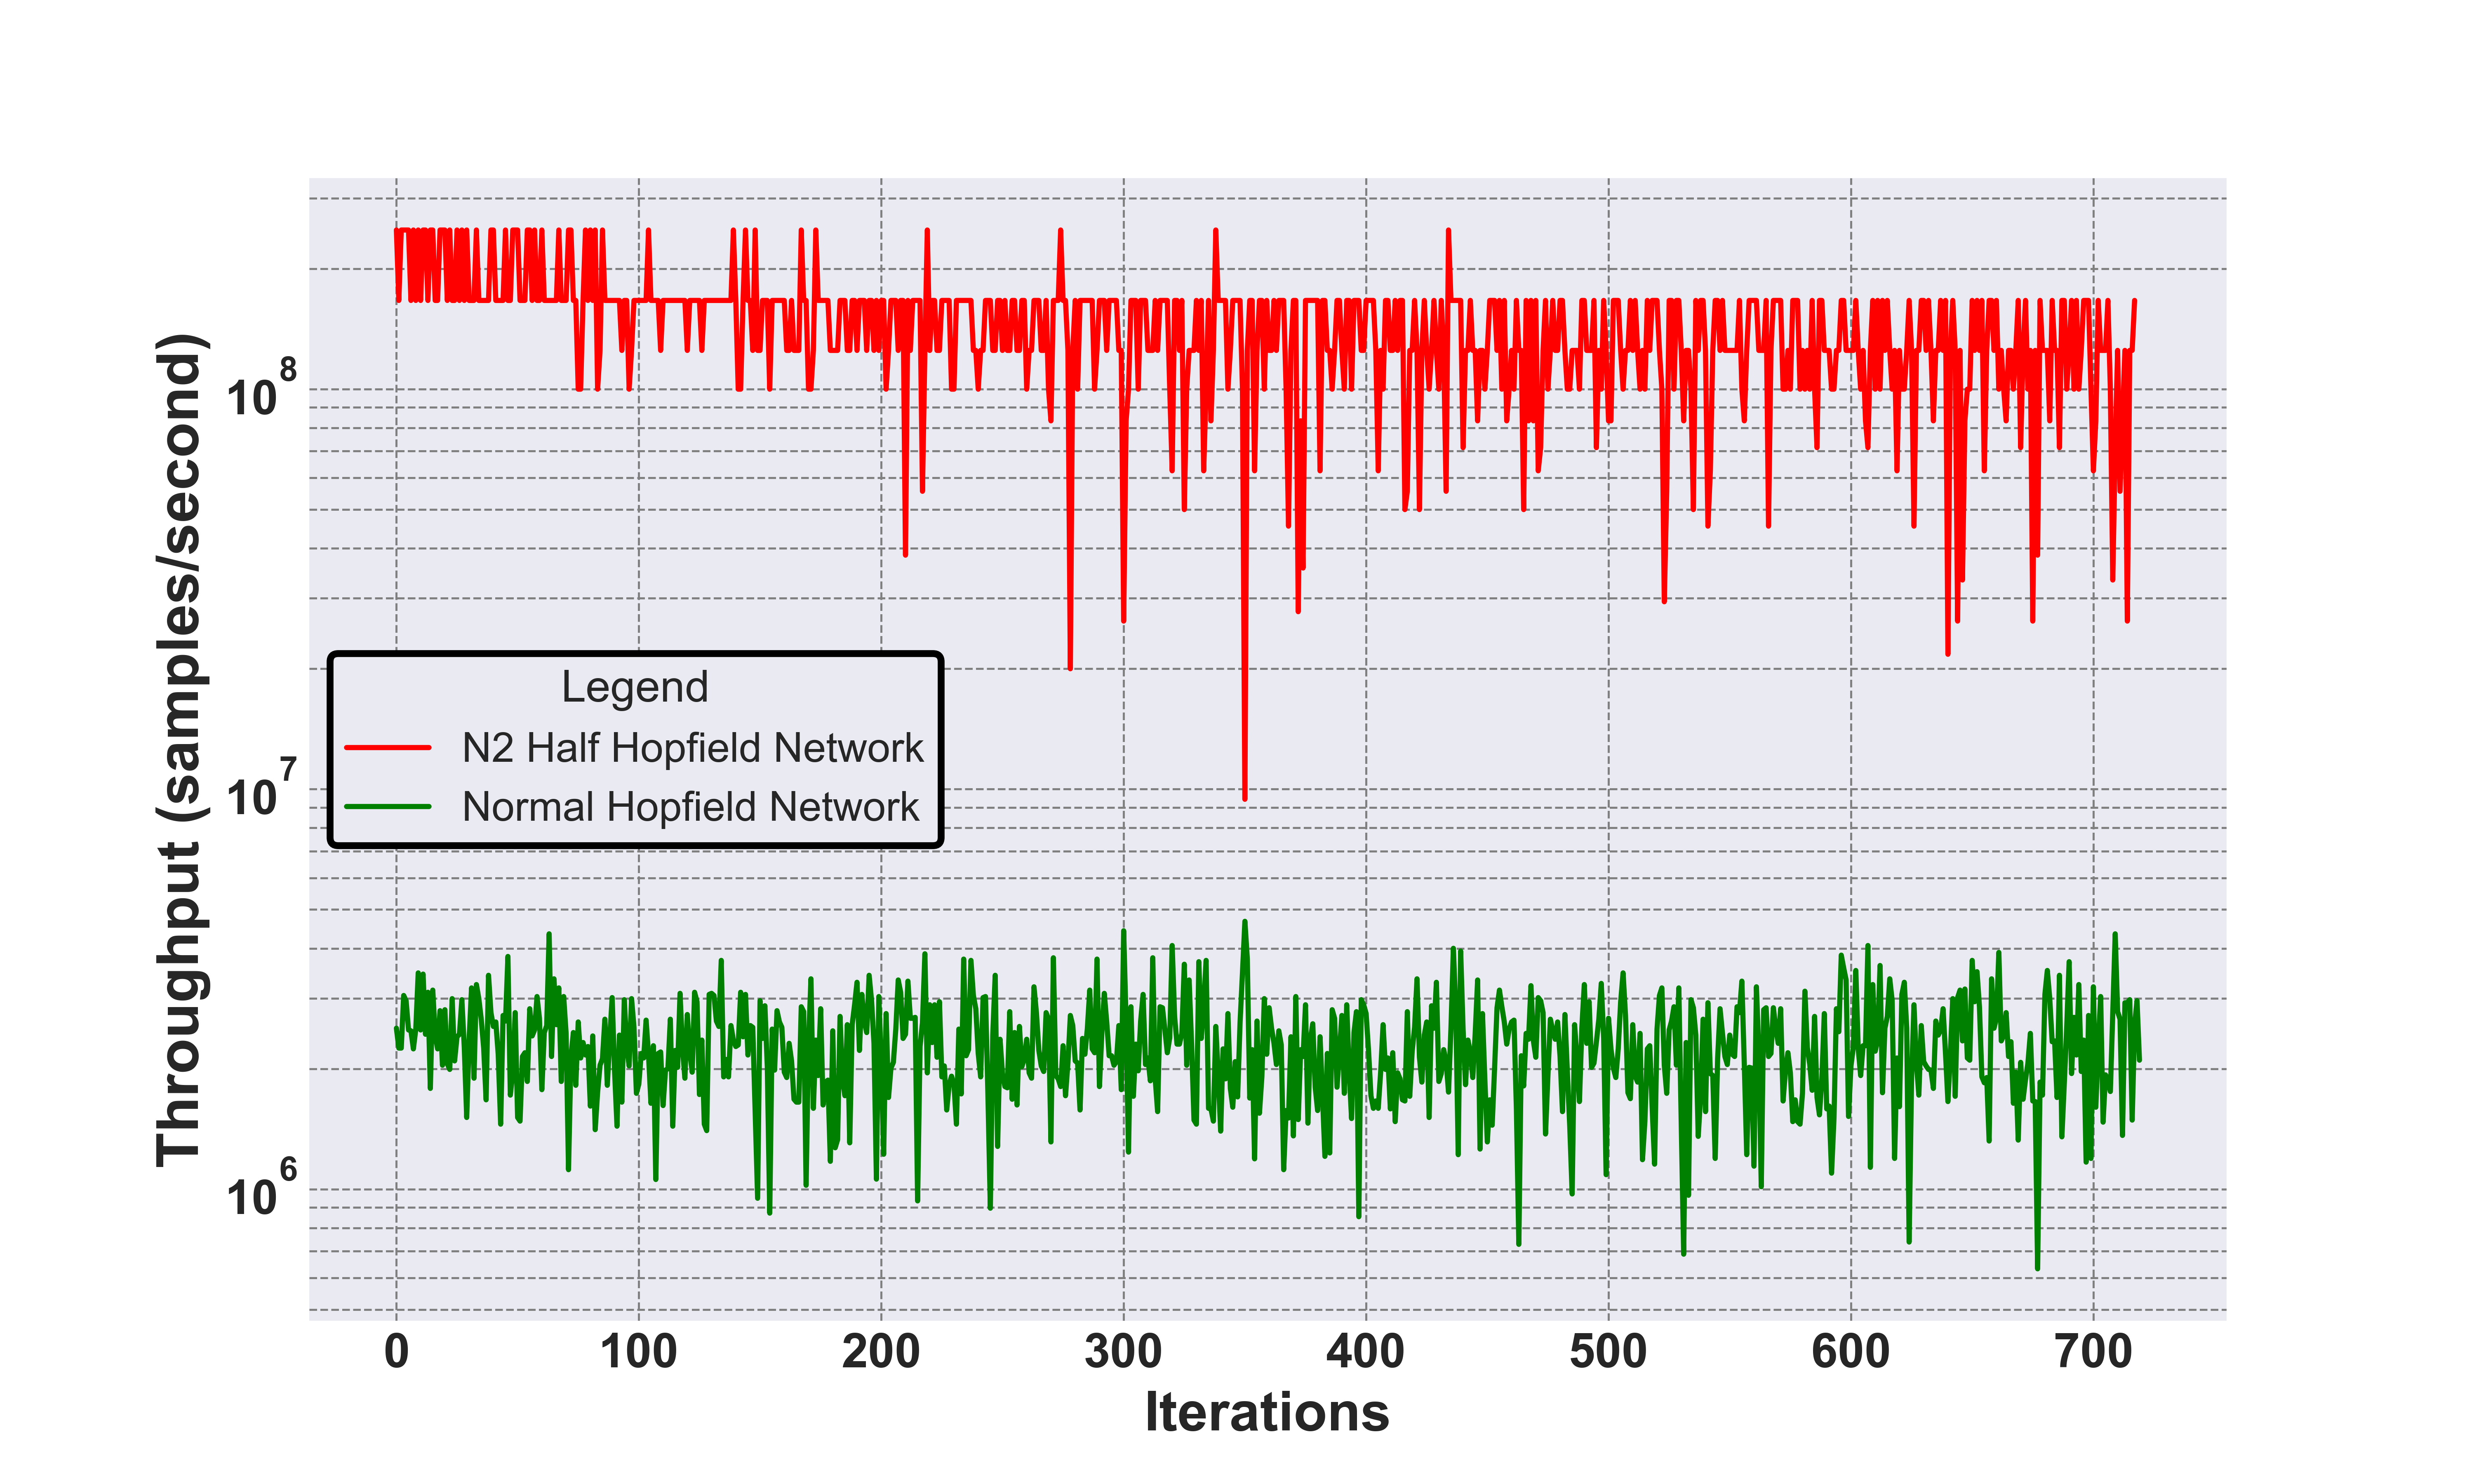
\includegraphics[width=0.8\linewidth]{graphics/Visualisierungen_throughput_log_2.png}
    \caption{throughput}
    \label{Throughput comparison}
\end{figure}
The following results can be gathered when comparing the two lines in terms of efficiency and stability:
The Normal Hopfield Network (green line) displays a stable throughput performance throughout the iterations, consistently above \(\mathbf{10^6}\)
samples per second. This suggests a stable and predictable behavior.
The N2 Half Hopfield Network (red line) exhibits significant variability in throughput. 
While it generally hovers around \(\mathbf{10^8}\) \textbf{to} \(\mathbf{10^9}\) the throughput is more sensitive and fluctuates more compared to the single update approach. 
To get a better feeling of the data, the average of the throughput is calculated: N/2 Half Hopfield Network has
an average of \textbf{144 megasamples/second}, while the
Normal Hopfield Network has an average of: \textbf{2,3 megasamples/second}. 
This means that the computation speed of the N/2 Half method \textbf{is faster} by a factor of \textbf{62.72x}.
Also in the attachment\ref{attachement:throughput_errors} is a version with the outliers included symolizing a throughput of zero for these two iterations.

The results of the autocorrelation implies a low computing time and low energy consumption than with conventional hardware.
To confirm this theory, the second metric to simulate is the \textbf{energy consumption} in energy/operation. 
Hence, the mentioned energy model needs to be implemented into the Hopfield Network interface.
The first adaptation is to \textbf{intialize the energy model} with the size of the neural network (164) as it impacts the size of the crossbar array and influences the overall energy consumption.
An increase in the number of neurons causes a higher energy consumption due to the enlarged crossbar structure.

Afterwards, the two parameters ``a\_pattern'' and ``a\_WL'' need to be calculated.
Hereby, a\_pattern refers to the currents that flow through the respective bitlines.
The current for each bitline is determined by the average of the weighted sum and is accumulated with each iteration.
Subsequently, it is divided by the number of sampling iterations to obtain an average for the respective training iteration.
For an correct calculation and imitation of the \ac{mem-HNN}, there is one more restriction to solve. 
The digital computer generates negative and positive weights and biases, which is not possible in the hardware.
Therefore, the weight matrix needs to be adjusted to handle positive and negastive weights seperately. 
Specifically, the weight matrix is discretized to the according bit resolution of the \ac{mem-HNN}, which is 5bit.
In the ealier design phases, the values were calculated with perfect resolution but for the energy model of the accelerator this is possible. 
Despite the low bit resolution there are many papers that proof that even with a small resolution a good performance can be achieved.\footnote{cf.\cite{maEra1bitLLMs2024}, p. 1; cf.\cite{GitHubHtqinQuantSR}, p. 1; cf.\cite{rouhaniMicroscalingDataFormats2023}, p. 1; cf.\cite{rouhaniSharedMicroexponentsLittle2023}, p. 1}
Since only positive weights can exist within the accelerator, these are separated and written into their own matrix.
This modification is essential to accommodate the hardware constraints that prevent the use of negative weights.

On the other hand, A\_Wl is the average configuration change.
This means This parameter tracks the average changes in configuration within the wordline.
Each time the state changes from 0 (no current) to 1 (current flows), energy is consumed to initially let the metal ions flow.
Therefore, every position in the configuration must be compared with the following configuration position wise.
Subsequently, an average change rate is calculated by dividing by the number of iterations.
This approach quantifies the energy cost associated with state transitions within the network configuration.
An estimate for this, especially for N/2 half is that 25\% of the neurons are updated in one training iteration (50\% randomly drawn and 50\% of that updated).
All the adjustments for the energy model to the interface can be found in the version 5 of the hopfield interface as part of the digital delivery.
The result of the energy consimption is illustrated in following figure\ref{Energy output_2}:
\begin{figure}[H]
    \centering
    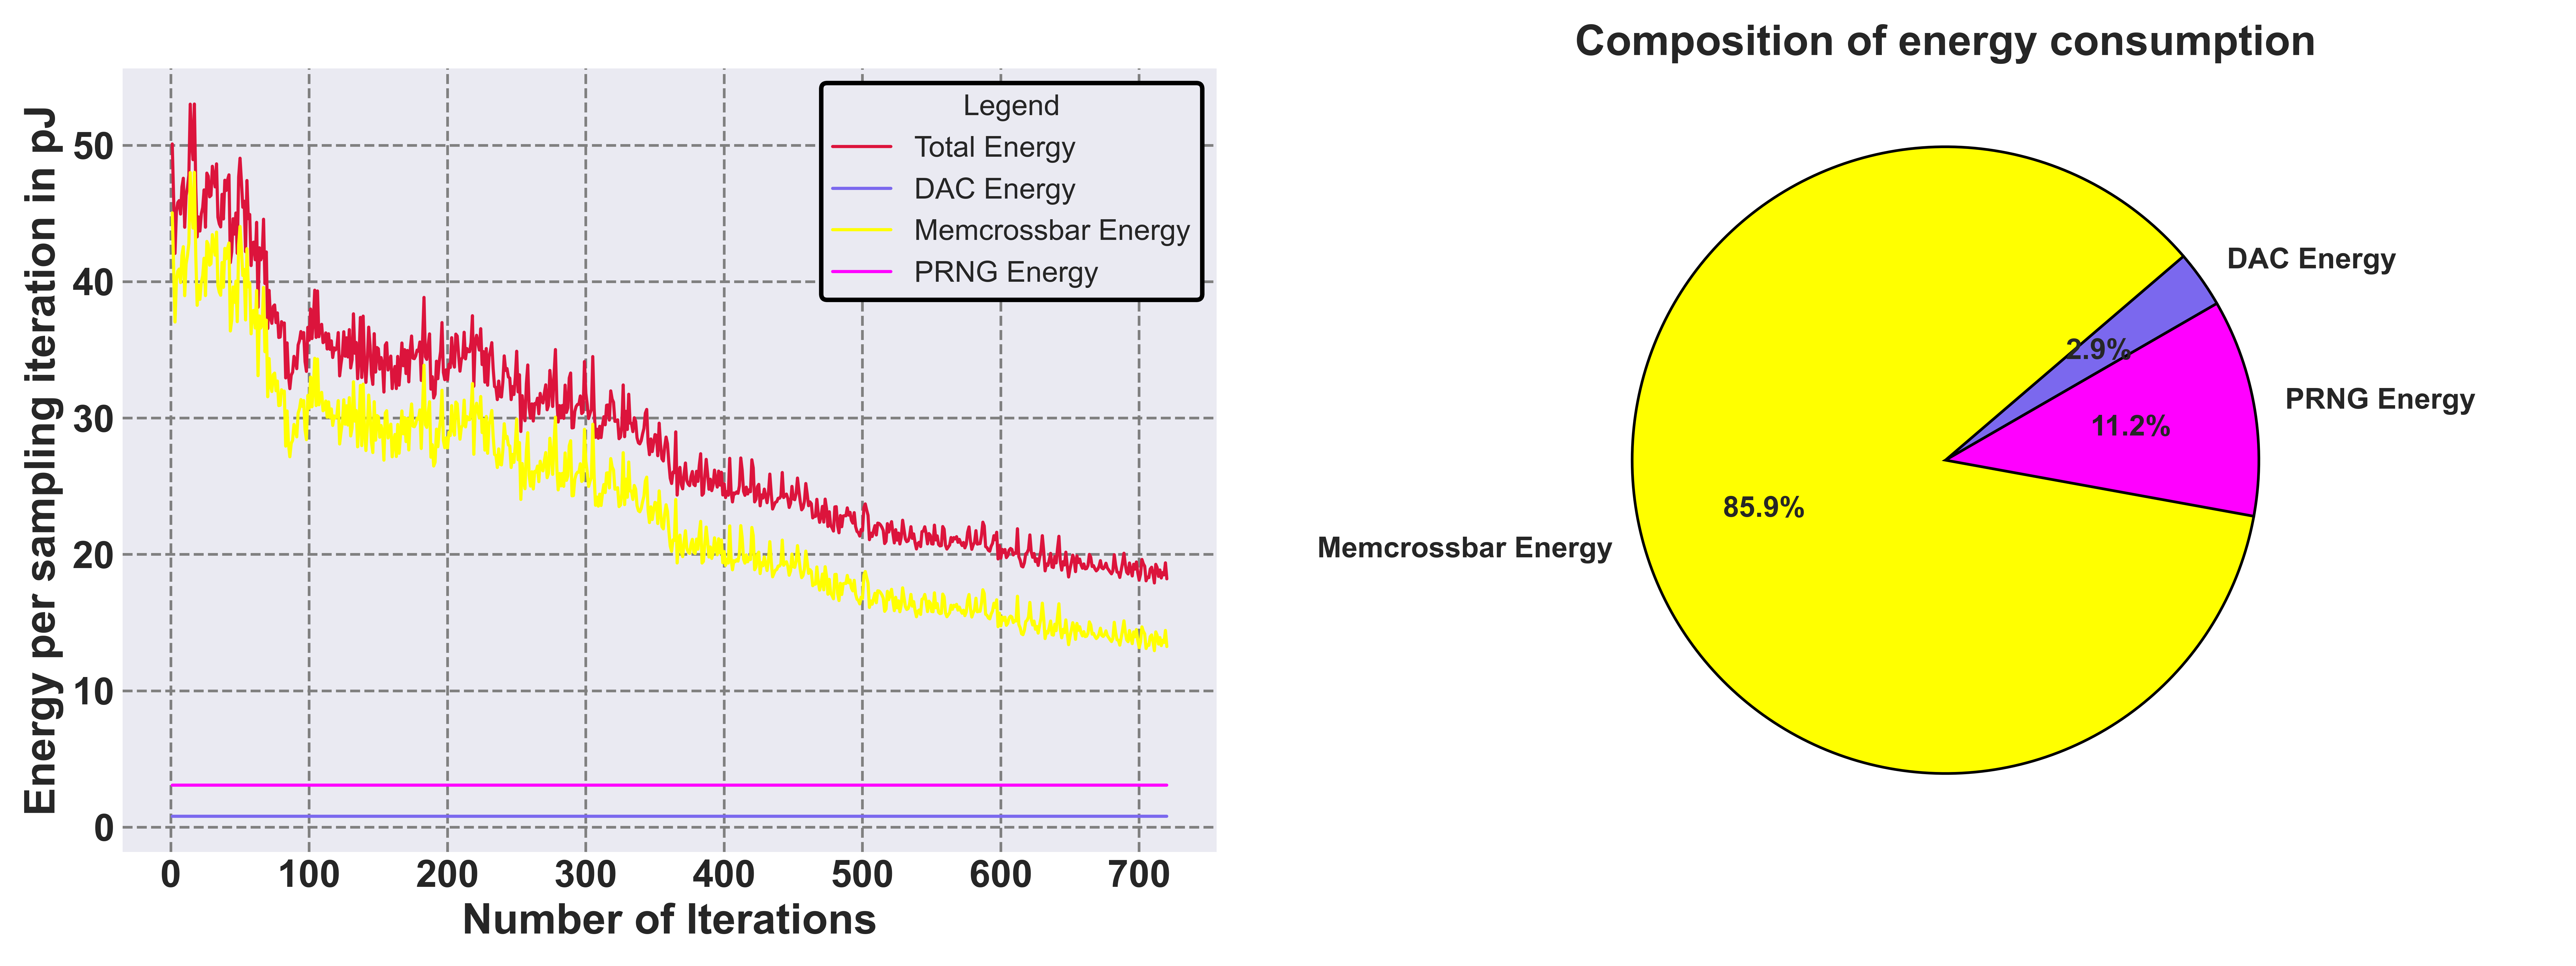
\includegraphics[width=1\linewidth]{graphics/energy_and_averages_plot_4.png}
    \caption{Energy consumption of the \ac{mem-HNN}}
    \label{Energy output_2}
\end{figure}
The left plot shows the energy consumed per sampling iteration (eq.\ to 1 clock cylce of the \ac{mem-HNN}) in piko Joules.
In the beginning of the training the average clock cycle has an total energy consumption of around 45 piko Joules.
Further in the training at atround 100 training iterations the consumption drops to around 35 piko Joules. 
In the end of the training the value falls just below the 20 piko Joules mark. 
The decrease of the energy consumption over the time comes from the weights of the neural netowotk that get better and better configured over time.
Noteworthy, the Memcrossbar energy is the only variable energy consumer that actively changes, while the digital-to-analog converter and the pseudo-random number generator stay horizontal.
A composition of the energy consumption is shown in the right plot.
Here 85\% of the energy is consumed entirely by the Memristor Crossbar and the support entities consume around 15\% of the energy.
The results of the energy model an the energy consumption can be verified by the following paper.\footcite[cf.][4]{hizzaniMemristorbasedHardwareAlgorithms2023}

Finally, it is important to mention that not all hardware components are included. and especially the communication and updating of 
For example the memory and the controller of the \ac{mem-HNN} and are not included in the plot.
Also to consider are the weights in the digital computer, that probably consume 10x the energy of the training on the analog \ac{mem-HNN}. 

In a next step the power consumption of the training is targeted as this delivers a good comparison to other
hardware components like \ac{CPU}s, \ac{GPU}, \ac{ASIC}s or \ac{FPGA}s.
Therefore, the energy per sampling iteration is divided by the time of one clock cycle (2ns) since \(P = \frac{\Delta E}{\Delta t}\).
Furthermore, the right plot is based on the power and cumulates the power multiplied with the sampling iteration to vissualize how much energy the training the neural network consumes for this workload.
\begin{figure}[H]
    \centering
    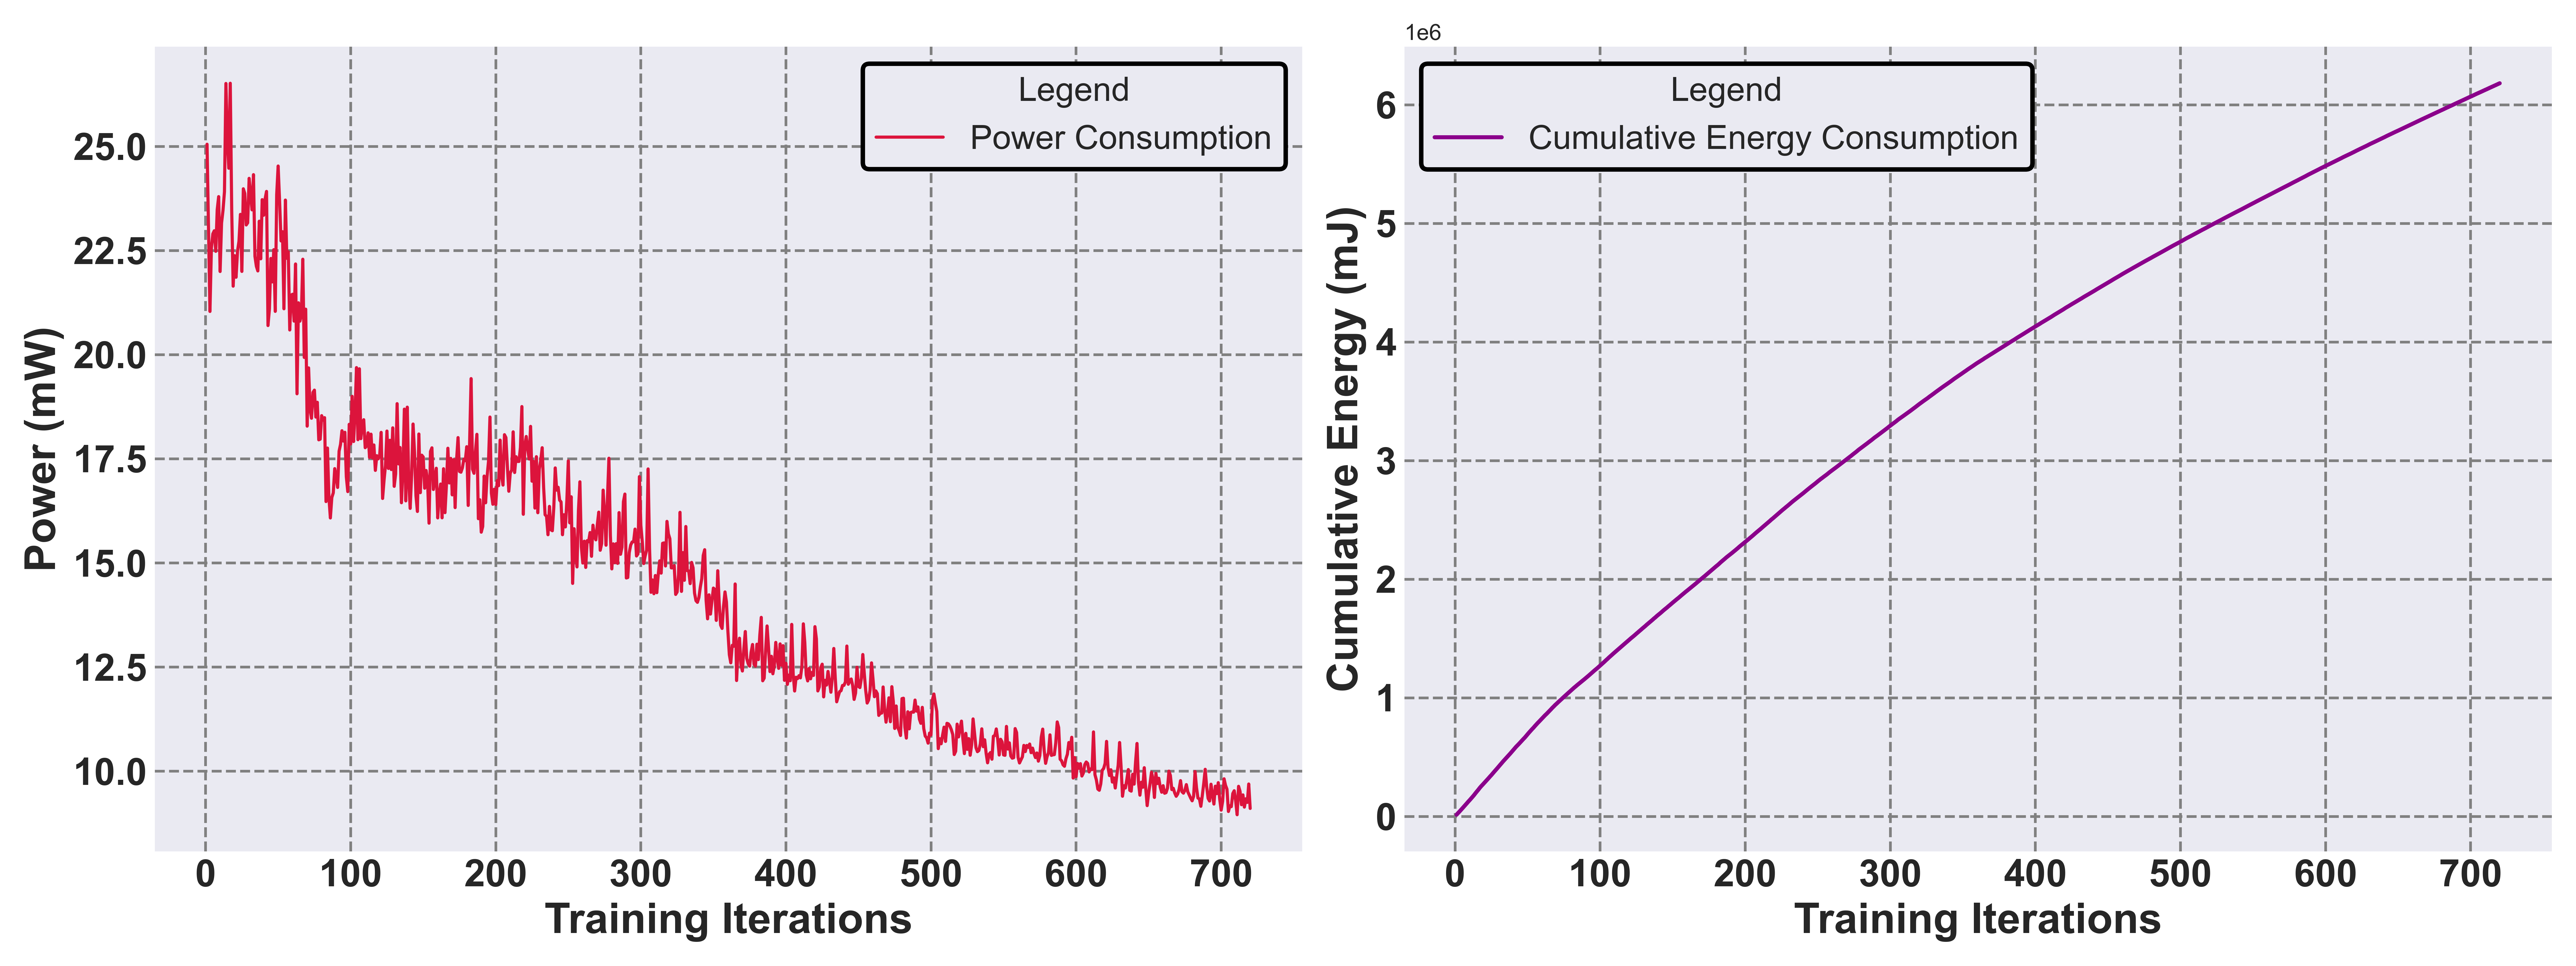
\includegraphics[width=1\linewidth]{graphics/energy_consumption_cumulative_plot.png}
    \caption{Power consumption of the \ac{mem-HNN}}
    \label{Power consumption}
\end{figure}
As shown in figure\ref{Power consumption} the power required to train is around 22.5 mW, which compared to a basic CPU(20-40W)
is significant less. 
Again with training iterations continuing to grow the power consumption decreases. 
At the end of the training around 620 iterations, an power consumption of around 10mW is reached. 
The entire power consumption is mostly stable with some larger fluctuatins in the beginning of the training areound 0 to 70 iterations.
When looking at the right plot, which symbolizes the cumulative energy required for the training in mJ.
Here, it is visible that a complete training with 720 iterations requires around 6.2 mJ. 
Again it is important to keep in mind that these numbers consist of only the \ac{mem-HNN} and do not include the digital computer.                                                                  	                                                                                                                                                                                                                                                                                                                                                                                                                                                                                                                                                                                                                                                                                                                                                                                                                                                                                    

With that the evaluation phase can successfully verify that the models purpose of the simulation, which is to answer the reasearch question, is achieved.
Therefore, Boltzmann Machines can indeed be efficiently implemented on the physics-inspired Hardware accelerator by analog noise injection. 